

\begin{figure}[hbt]
	\centering
	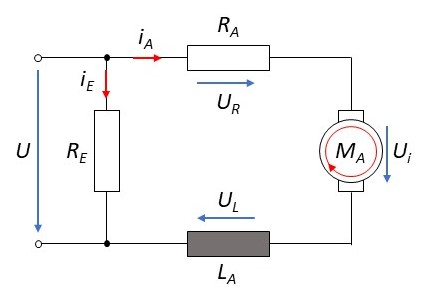
\includegraphics[width=0.5\linewidth]{Images/ProjektB_Elektrik_Ph_Modell_Schaltplan}
	\caption{Physikalisches Modell mit Spannungen und Strömen}
	\label{fig:schaltbild}
\end{figure}

Zu den elektrischen Größen:
\begin{equation*}
\begin{aligned}
&M_A = K_A i_A \\
&P_A = U_i i_A = M_A \omega_A = K_A i_A \omega_A \\
&U_i = K_A \omega_A = K_A \dot{\varphi} \\
&i_E = \frac{U}{R_E}
\end{aligned}
\end{equation*}

Mathematisches Modell der Nebenschlussmaschine:
\begin{equation*}
\begin{aligned}
&U = U_R + U_i + U_L \\
&U = R_A i_A + K_A \dot{\varphi} + L_A \frac{\diff{i_A}}{\diff{t}} \\
&0 = R_A i_A + K_A \dot{\varphi} + L_A \frac{\diff{i_A}}{\diff{t}} - U \\
\end{aligned}
\end{equation*}

Systemgleichung des Umwuchtsystems:
Translatorisch:
\begin{equation}
\begin{aligned}
(m_1 + m_2) \ddot{s} - m_2 e(\ddot{\varphi} \sin{\varphi} + \ddot{\varphi^2} \cos{\varphi}) + d_t \dot{s} + c s &= 0 \\
\ddot{s} = \frac{1}{m_1 + m_2}[m_2 e(\ddot{\varphi} \sin{\varphi} + \ddot{\varphi^2} \cos{\varphi}) - d_t \dot{s} - c s] &= f_1(\varphi, \dot{\varphi}, \ddot{\varphi}, s, \dot{s}) \label{enq:Bewgltrans}
\end{aligned}
\end{equation}
Rotatorisch:
\begin{equation}
\begin{aligned}
m_2 e^2 \dot{\varphi} - m_2 e \sin{\varphi} (\ddot{s} + g) d_r \dot{\varphi} - M_A &= 0 \\
m_2 e^2 \dot{\varphi} - m_2 e \sin{\varphi} (\ddot{s} + g) d_r \dot{\varphi} - K_A i_A &= 0 \\
\ddot{\varphi} = \frac{1}{m_2 e^2} [m_2 e \sin{\varphi} (\ddot{s} + g) d_r \dot{\varphi} + K_A i_A] &= f_2(\varphi, \dot{\varphi}, \ddot{s}, i_A) \label{enq:Bewglrot}
\end{aligned}
\end{equation}

Durch Vernachlässigung des Erregerstroms $i_E$ folgt:
\begin{equation}
\begin{aligned}
U &= i_A R_A + L_A \dot{i_A} + K_A \dot{\varphi} \\
\frac{\diff{i_A}}{\diff{t}} &= \frac{1}{L_A} (U - K_A \dot{\varphi} - i_A R_A) = f_3(U, \dot{\varphi}, i_A)
\end{aligned}
\end{equation}

%Folgesituationen
\begin{figure}[hbt]
	\begin{tikzpicture}
	
	%Zeichnung de Holzblöcke
	\draw (4,0.5) rectangle (9,2.5) node[midway, align=center](Block){Unwuchtsystem}; 
	
	%Pfeile
	\begin{scope}
	\draw[->] (0,1.5) -- (4,1.5);
	\draw[->] (9,1.5) -- (13,1.5);
	\end{scope}
	
	%Parameterbeschriftungen
	\draw(0,2.25) node(uin) {$u = U$};
	\draw(13.75,2.25) node(yvek) {$\underline{y} = \left[\begin{array}{c} s \\\ \dot{\varphi} \\\ M_A \\\ F_U \end{array}\right]$};
	
	\end{tikzpicture}
	
	%Abbildungsunterschrift
	\caption{Unwuchtsystem mit Eingangsspannung und Ausgang (Kinematik, Kinetik)}
	\label{fig:Unwuchtsystem}
	
\end{figure}


\begin{figure}[hbt]
	\centering
	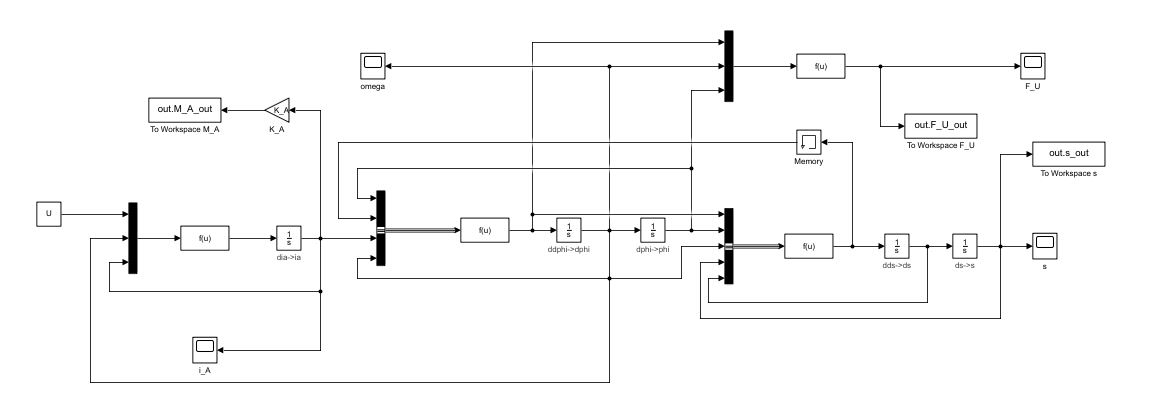
\includegraphics[width=1\linewidth]{Images/ProjektB_Elektrik_Blockdiagramm}
	\caption{SIMULINK Blockdiagramm zur Simulation des Systemverhaltens mit Memory-Block zur Umgehung der algebraischen Schleife}
	\label{fig:Blockdiagramm}
\end{figure}

\begin{figure}[hbt]
	\centering
	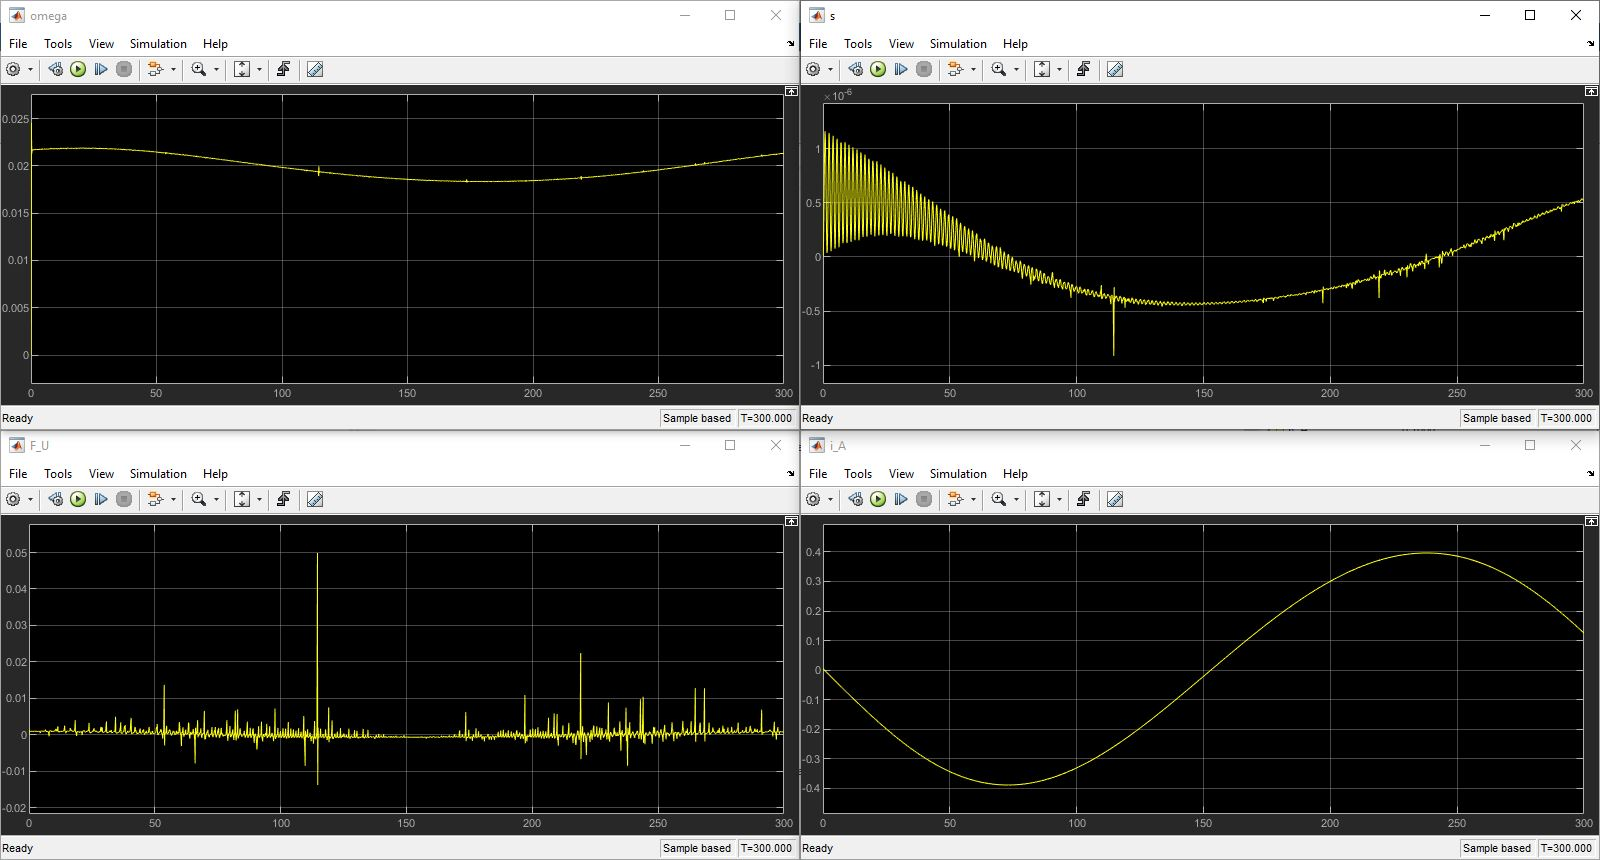
\includegraphics[width=0.5\linewidth]{Images/ProjektB_Elektrik_Diagramme_1}
	\caption{Simulationsergebnisse}
	\label{fig:Simulationsergebnisse}
\end{figure}
